\documentclass[12pt]{book}
\usepackage{amsmath, amssymb, amsthm}
\usepackage{latexsym, epsfig, ulem, cancel, multicol, hyperref}
\usepackage{graphicx, tikz, subfigure,pgfplots}
\usepackage{blindtext}
\usepackage[a4paper, total={6in, 8in}]{geometry}
\setlength{\parindent}{0pt}
\usepackage{multirow}
\usepackage{mathtools}
\pgfplotsset{width=10cm,compat=1.9}
\usepackage{amsmath, amssymb, amsthm, graphicx, hyperref}
\usepackage{enumerate}
\usepackage{fancyhdr}
\usepackage{multirow, multicol}
\usepackage{tikz}
\usepackage{comment}
\setlength{\parskip}{1ex}

\newcommand{\T}[0]{\top}
\newcommand{\F}[0]{\bot}
\newcommand{\liminfty}[1]{\lim_{#1 \to \infty}}
\newcommand{\limzero}[1]{\lim_{#1 \to 0}}
\newcommand{\limto}[1]{\lim_{#1}}
\newcommand{\Z}{\mathbb{Z}}
\newcommand{\R}{\mathbb{R}}
\newcommand{\C}{\mathbb{C}}
\newcommand{\Q}{\mathbb{Q}}
\newcommand{\odd}[0]{\mathbb{Z} - 2\mathbb{Z}}
\newcommand{\lineint}[1]{\int_{#1}}
\newcommand{\pypx}[2]{\frac{\partial #1}{\partial #2}}
\newcommand{\divg}{\nabla \cdot}
\newcommand{\curl}{\nabla \times}
\newcommand{\dydx}[2]{\frac{d #1}{d #2}}
\newcommand{\sqbkt}[1]{\left[ #1 \right]}
\newcommand{\paren}[1]{\left( #1 \right)}
\newcommand{\tribkt}[1]{\left< #1 \right>}
\newcommand{\abso}[1]{\left|#1 \right|}
\newcommand{\zero}{\{0\}}
\newcommand{\then}{\rightarrow}
\newcommand{\nonneg}{\Z^+ \cup \{0\}}
\DeclarePairedDelimiter\ceil{\lceil}{\rceil}
\DeclarePairedDelimiter\floor{\lfloor}{\rfloor}
\newcommand{\union}[2]{\bigcup_{#1}^{#2}}
\newcommand{\inter}[2]{\bigcap_{#1}^{#2}}
\newcommand{\openclose}[1]{\left( #1 \right]}
\newcommand{\closeopen}[1]{\left[ #1 \right)}
\newcommand{\compo}[2]{#1 e^{i #2}}

\newtheorem*{remark}{Remark}
\title{\textbf{Complex Variable and Linear Algebra}}
\author{Dennis Li}
\begin{document}
\maketitle

\tableofcontents

\chapter{Intro to Complex Numbers}

\section{The complex number}
\subsection{Definition}
A complex number is defined as follows for some real number $a,b$
\begin{align}
    z = a+ib
\end{align}
Where the letter $i$ here is defined as follows
\begin{align}
    i = \sqrt{-1}
\end{align}
We define the following operation on a complex number.
\begin{align}
    Re(z) = a\\
    Im(z) = b
\end{align}
Where $Re$ extracts the real part of $z$ and $Im$ takes the imaginary part of $z$, that is, the coefficient of $i$. Note that the $Im$ operation does not include the number $i$. We use the symbol $\C$ to represent the set of all complex number. It is a superset of $\R$, the set of all real numbers. 
\subsection{Conjugate}
The conjugate of a complex number $z = a+ib$ is defined as follows
\begin{align}
    \Bar{z} = a - ib
\end{align}
Where you simply flip the sign of the imaginary part of the complex number. And the conjugate of a complex number is denoted as $\Bar{z}$.
\subsection{Modulus}
The modulus of a complex number is defined as follows
\begin{align}
    \abso{z} = \sqrt{z\Bar{z}}
\end{align}
If we expand and simplify, we have
\[
z\Bar{z}=(a+bi)(a-bi) = a^2 - (ib)^2 = a^2+b^2
\]
Therefore the modulus of a complex number is actually
\begin{align}
    \abso{z} = \sqrt{a^2 + b^2}
\end{align}



\section{Elementary Operation on Complex Number}
\subsection{Addition and Multiplication}
The addition and subtraction of complex number are straight forward. If we define 2 complex numbers $z_1 = a+ib$ and $z_2 = c+id$, then
\begin{align}
    z_1+z_2 = (a+c)+i(b+d)
\end{align}
Similarly for subtraction. And multiplication can be defined as
\begin{align}
    z_1z_2 = (a+bi)(c+di) = ac + dbi^2 + adi + cbi = (ac-db)+i(ad+cb)
\end{align}
And example being
\begin{align}
    (3+4i)(-1-6i) = -3-18i-4i+24 = 21-22i
\end{align}
\subsection{Division}
The division between complex numbers can be carried out as follows.
\begin{align}
    \frac{z_1}{z_2} = \frac{a+ib}{c+id} 
\end{align}
To obtain the result, we want to make the denominator real, so we can rewrite the fraction. There are 2 approach. 
\subsubsection{First approach}
We set the fraction equal to a generic complex number
\begin{align}
    \frac{a+ib}{c+id}  = x+iy
\end{align}
And we will solve it as a system of equations, and obtain 2 solutions for $x$ and $y$ where you have to eventually find the right pair. This method is not recommended. 
\subsubsection{Second Approach}
In this method, we simply multiply the denominator by its conjugate, this will give us a real denominator that allows us to rewrite the fraction. 
\begin{align}
    \frac{a+ib}{c+id} = \frac{(a+ib)(c-id)}{c^2+d^2}
\end{align}
Since $c^2 + d^2$ is a real number, first simplify the numerator and then distribute the denominator into each term to obtain the final result. An example being:
\begin{align*}
    \frac{1+2i}{2+i} &= \frac{(1+2i)(2-i)}{(2+i)(2-i)}\\
                     &= \frac{2 - i + 4i + 2}{4+1}\\
                     &= \frac{4+3i}{5}\\
                     &=\frac{4}{5}+\frac{3}{5}i
\end{align*}

\newpage
\section{Polar Form of Complex Number}
\subsection{Euler's Identity}
Before we start, we can go through how this great equation is derived.
\[
e^{i\theta} = \cos\theta+i\sin\theta
\]
First we would recall the Taylor series expansion of $e^{ax}$ as follows
\[
e^{ax} = \sum_{n=0}^{\infty} =1 + ax + \frac{a^2x^2}{2!}+ \frac{a^3x^3}{3!}\ldots
\]
And if we are to replace $a$ with the imaginary number, which is also a constant, $i$, we have
\[
e^{ix} = \sum_{n=0}^{\infty} =1 + ix + \frac{i^2x^2}{2!}+ \frac{i^3x^3}{3!}+\frac{i^4x^4}{4!}\ldots
\]
But we know by definition that $i^2 = -1$, $i^3 = -i$, and $i^4=1$, we can simplify
\[
e^{ix} = \sum_{n=0}^{\infty} =1 + ix - \frac{x^2}{2!} - \frac{ix^3}{3!} + \frac{x^4}{4!} \ldots
\]
Now if we look remember the Taylor series expansion of $\cos x$ and $\sin x$, we have
\[
\cos x = \sum_{n=0}^{\infty} \frac{(-1)^n x^{2n}}{(2n)!} = 1 - \frac{x^2}{2!} + \frac{x^4}{4!} - \frac{x^6}{6!} + \ldots
\]
\[
\sin x = \sum_{n=0}^{\infty} \frac{(-1)^n x^{2n+1}}{(2n+1)!} = x - \frac{x^3}{3!} + \frac{x^5}{5!} - \frac{x^7}{7!} + \ldots
\]
Since $i$ is a constant, we can simply multiply it to $\sin x$, and obtain
\[
i\sin x = i\sum_{n=0}^{\infty} = ix - \frac{ix^3}{3!} + \frac{ix^5}{5!} - \frac{ix^7}{7!} + \ldots
\]
Notice that we can regroup the terms of $e^{ix}$
\[
e^{ix} = \left(1 - \frac{x^2}{2!} + \frac{x^4}{4!} - \frac{x^6}{6!} + \ldots \right) + i \left(x - \frac{x^3}{3!} + \frac{x^5}{5!} - \ldots \right).
\]
This in turn shows that
\[
e^{ix} = \cos x + i\sin x
\]

\subsection{The complex Plane}

\begin{figure}[!h]
    \centering
    \begin{tikzpicture}
        \begin{axis}[
            axis lines = middle,
            xlabel = {Real},
            ylabel = {Imaginary},
            xlabel style = {below right},
            ylabel style = {above left},
            xtick = {-3, -2, -1, 0, 1, 2, 3},
            ytick = {-3, -2, -1, 0, 1, 2, 3},
            yticklabels = {$-3i$, $-2i$, $-i$, $0$, $i$, $2i$, $3i$},
            xmin = -3.5, xmax = 3.5,
            ymin = -3.5, ymax = 3.5,
            width = 12cm, height = 12cm,
            enlarge x limits = 0.15,
            enlarge y limits = 0.15,
        ]
        % Adding the point (1, 1) which corresponds to 1+i
        \addplot[
            only marks,
            mark=*,
            mark options={fill=red,draw=black}
        ] coordinates {(1,1)};
        
        % Adding a label for the point 1+i
        \node[label={above right:{\scriptsize $1+i$}},circle,fill,inner sep=1.5pt] at (axis cs:1,1) {};
         % Adding the vector from (0,0) to (-1,2)
        \addplot[
            ->, % Arrow style
            thick, % Thickness of the line
            color=blue % Color of the vector
        ] coordinates {(0,0) (-1,2)};
        
        % Adding a label for the point -1+2i
        \node[label={above:{\scriptsize$-1+2i$}},circle,fill,inner sep=1.5pt] at (axis cs:-1,2) {};
        % Adding the vector for -2+i
        \addplot[
            ->, % Arrow style
            thick, % Thickness of the line
            color=red % Color of the vector
        ] coordinates {(0,0) (-2,1)};
        
        % Label for -2+i
        \node[label={above left:{\scriptsize$-2+i$}},circle,fill,inner sep=1.5pt] at (axis cs:-2,1) {};
        
        % Adding the vector for the sum (-3+3i)
        \addplot[
            ->, % Arrow style
            thick, % Thickness of the line
            color=green % Color of the vector
        ] coordinates {(0,0) (-3,3)};
        
        % Label for the sum -3+3i
        \node[label={above left:{\scriptsize$-3+3i$}},circle,fill,inner sep=1.5pt] at (axis cs:-3,3) {};
         % Vector from tip of -2+i to tip of -3+3i, indicating the addition
        \addplot[
            ->, % Arrow style
            dashed, % Dashed line style
            thick, % Thickness of the line
            color=purple % Color of the vector
        ] coordinates {(-2,1) (-3,3)};

    
        \end{axis}
    \end{tikzpicture}
    \caption{Representation of complex numbers in a complex plane}
    \label{fig:1.1}
\end{figure}

Above is the complex plane, which is basically a Cartesian plane where the $y$ axis is multiplied by $i$. Think of it like a Cartesian plane that is composed of $\R \times i\R$.

You can effectively represent all complex number as a point on the complex plane with its real part as the $x$ coordinate and the imaginary part as the $y$ coordinate. In the graph, we plotted $1+i$ on the coordinate $(1,1)$.

Another way to think of complex number is to think of it as a vector from the origin to the point where the complex number resides. The advantage of thinking it like this is, it makes addition of complex number more intuitive as it coincides with the addition of vectors on a 2D plane. You can see the example in the same graph above. 
\newpage
Thinking of them like a vector also makes modulus more intuitive, since it is defined similarly to the magnitude of a vector. (Even the symbol is the same.) And if we were to draw all complex number that has the modulus of $1$, that is $\abso{z} = 1$, we would obtain something very familiar.

\begin{figure}[!h]
    \centering
    \begin{tikzpicture}
        \begin{axis}[
            axis lines = middle,
            xlabel = {Real},
            ylabel = {Imaginary},
            xlabel style = {below right},
            ylabel style = {above left},
            xtick = { -1, 0, 1},
            ytick = { -1, 0,  1},
            yticklabels = { $-i$, $0$, $i$},
            xmin = -1.3, xmax = 1.3,
            ymin = -1.3, ymax = 1.3,
            width = 7.5cm, height = 7.5cm,
            enlarge x limits = 0.15,
            enlarge y limits = 0.15,
            axis equal, % Ensures the aspect ratio is 1:1
        ]
        
        % Drawing the unit circle |z| = 1
        \addplot[
            domain=0:360,
            samples=100,
            thick,
            color=blue,
        ] ({cos(x)}, {sin(x)});
        
        % Label for the unit circle
        \node[label={right:{\scriptsize $|z| = 1$}}] at (axis cs:1,1) {};
        
        \end{axis}
    \end{tikzpicture}
    \caption{The graph of the unit circle in the complex plane}
    \label{fig:1.2}
\end{figure}

After familiarizing ourselves with expressing complex number as a point on the complex plain, we can try to express it in a different form. 
\begin{figure}[!h]
    \centering
    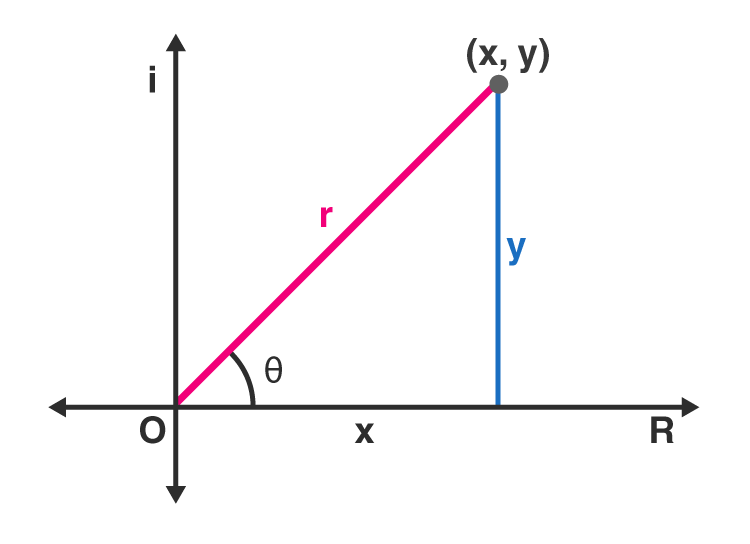
\includegraphics[width=0.5\linewidth]{pictures/pic1.3.1.png}
    \caption{A complex number $z = x+iy$}
    \label{fig:1.3}
\end{figure}
Given a complex number $z = x+iy$, we can plot it on the complex plane as shown above. Where $r$ is the distance from the origin, or the modulus of the complex number, and $\theta$ the angle of the supposed \textit{vector} with the real axis. 

\subsection{Argument of a Complex Number}
\subsubsection{Principle Argument}
The angle $\theta$ this supposed vector make with the real axis is called the \textbf{principle argument} of the complex number, the principle argument of the complex number $z$ is denoted as $Arg(z)$. For example, the argument of the complex number $1+i$ would be 
\begin{align}
    Arg(1+i) = \tan^{-1}\paren{\frac{1}{1}} = \frac{\pi}{4}
\end{align}
The range of the principle argument is $\theta \in \openclose{-\pi,\pi}$. There are some minor details that require some care.
\begin{enumerate}
    \item if $z_{(1,4)}=a+ib$ is in the first and the fourth quadrant of the complex plane, the principle argument is simply the following
    \begin{align}
        Arg(z_{(1,4)}) = \tan^{-1}\paren{\frac{b}{a}}
    \end{align}
    \item if $z = a+ib$ is in the second quadrant, the principle argument requires some tweak
    \begin{align}
        Arg\paren{z_2} = \pi - \tan^{-1}\paren{\frac{|b|}{|a|}}
    \end{align}
    \item if $z_3=a+ib$ is in the third quadrant, the principle argument is
    \begin{align}
        Arg(z_3) = \tan^{-1}\paren{\frac{|b|}{|a|}} - \pi
    \end{align}
\end{enumerate}
These tweaks are done so it properly reflects the angle of the complex number and the real axis. 
\newpage
\subsubsection{Argument}
There is another way of defining the angle between the complex number and the real axis. It is simply called the \textbf{argument} of the complex number. Regardless of the angle of the principle argument, you can always rotate another $2\pi$ radian and return to the same position. Therefore there the \textbf{argument} of a complex number $z$ is defined slightly different from the principle argument. The argument of a complex number $z$ is denoted as $arg(z)$
\begin{enumerate}
    \item if $z_{(1,4)}=a+ib$ is in the first and the fourth quadrant of the complex plane, the argument is simply the following
    \begin{align}
        arg(z_{(1,4)}) = \tan^{-1}\paren{\frac{b}{a}} + 2\pi n \quad n \in \Z
    \end{align}
    \item if $z = a+ib$ is in the second quadrant, the argument requires some tweak
    \begin{align}
        arg\paren{z_2} = \pi - \tan^{-1}\paren{\frac{|b|}{|a|}} + 2\pi n \quad n \in \Z
    \end{align}
    \item if $z_3=a+ib$ is in the third quadrant, the argument is
    \begin{align}
        arg(z_3) = \tan^{-1}\paren{\frac{|b|}{|a|}} - \pi + 2\pi n \quad n \in \Z
    \end{align}
\end{enumerate}
What happens here is that you can add an arbitrary integer multiple of $2\pi$ and you will come back to the same location. Therefore there are infinitely many outcomes. 

\subsection{Polar Form of a Complex Number}
Going back to figure \ref{fig:1.3.1}, we now have a good definition for the angle (the argument) and the distance (the modulus) of a complex number. We can actually define a complex number using the idea of a polar coordinate system. Think of this unit circle $\abso{z} = 1$ in the complex plane. 

\begin{figure}
    \centering
    \begin{tikzpicture}
        \begin{axis}[
            axis lines = middle,
            xlabel = {Real},
            ylabel = {Imaginary},
            xlabel ={},
            ylabel ={},
            xtick = \empty,
            ytick = \empty,
            xmin = -1.5, xmax = 1.5,
            ymin = -1.5, ymax = 1.5,
            width = 7.5cm, height = 7.5cm,
            enlarge x limits = 0.15,
            enlarge y limits = 0.15,
            axis equal, % Ensures the aspect ratio is 1:1
        ]
        
        % Drawing the unit circle |z| = 1
        \addplot[
            domain=0:360,
            samples=100,
            thick,
            color=blue,
        ] ({cos(x)}, {sin(x)});
        
        % Plotting the complex number 1/sqrt(2) + i/sqrt(2)
        \addplot[
            ->, % Arrow style
            thick, % Thickness of the line
            color=red % Color of the vector
        ] coordinates {(0,0) (0.7071,0.7071)}; % 1/sqrt(2) is approximately 0.7071
        
        % Label for the complex number
        \node[label={above right:{\scriptsize $z = a + ib$}},circle,fill,inner sep=1.5pt] at (axis cs:0.7071,0.7071) {};
        
        \end{axis}
    \end{tikzpicture}
    \caption{The graph of $|z| = R$}
    \label{fig:1.4}
\end{figure}

Let $\abso{z} = R$ and $arg(z) = \theta$ . And we can in fact express the position of the given complex number on the graph as $z \colon \paren{R\cos \theta ,R\sin \theta}$, and the entire complex number as
\begin{align}
    z = R\cos \theta + iR\sin\theta
\end{align}
Recall the \textbf{Euler's Identity}
\begin{align}
    re^{i\theta} = r\cos\theta + ir\sin\theta
\end{align}
We can rewrite our complex number as
\begin{align}
    z = Re^{i\theta} \quad 
    \begin{cases}
        R = \abso{z}\\
        \theta = arg(z) \; \text{or} \; Arg(z)
    \end{cases}
\end{align}
This is called the \textbf{polar form} of a complex number. 
\subsubsection{Modulus in the Polar Form}
If we have a complex number in the form
\[
z = R\cos \theta + iR\sin\theta
\]
Its modulus would be, as defined previously
\[
\Bar{z} = R\cos \theta - iR\sin\theta
\]
Since cosine is an even function, and sine is an odd function we can manipulate it as follows
\[
\Bar{z} = R\cos \paren{-\theta} + iR\sin\paren{-\theta}
\]
With Euler's identity, we find that it is
\begin{align}
    \Bar{z} = Re^{-i\theta}
\end{align}
If we are to multiply the complex number $z$ with its conjugate, we have
\[
z\Bar{z} = \paren{Re^{i\theta}}\paren{Re^{-i\theta}} = R^2e^{i\theta-i\theta} = R^2
\]
Which matches our expectation from what we defined previously. and with the polar form of a complex number defined, we can now do more fancy operations on them.

\section{Powers of Complex Number}
We can now raise complex numbers to different powers with our new definition. The square of a complex number $z = Re^{i\theta}$ can simply be obtained by 
\begin{align}
    z^2 = \paren{Re^{i\theta}}^2 = R^2 e^{2i\theta}
\end{align}
Similarly, we can take the square root, or the $\frac{1}{2}$ power of $z$ as follows
\begin{align}
    \sqrt{z} = z^{\frac{1}{2}} = R^{\frac{1}{2}}e^{\frac{1}{2}i\theta}
\end{align}
Simply expanding it back to the expanded form, we will obtain
\begin{align}
    \sqrt{z} = \frac{R}{2}\cos\paren{\frac{\theta}{2}} + \frac{R}{2}i\sin\paren{\frac{\theta}{2}}
\end{align}
You can use this to define the $n$-th power of a complex number. 
\begin{align}
    z^n = R^n e^{ni\theta} = R^n\cos\paren{n\theta} + R^ni\sin\paren{n\theta}
\end{align}
Since the argument of a complex number can be manipulated freely by adding integer multiple of $2\pi$, we define the equality of 2 complex number $u,w \in \C$ as
\begin{align}
    u = w \iff
    \begin{cases}
        R_u = R_w\\
        \theta_u - \theta_w = 2\pi n \quad n \in \Z
    \end{cases}
\end{align}
\subsubsection{Example 1.4.1}
Here we provide an example of finding the square root of the complex number $z = 1+i$. First we would rewrite it in polar form, to do so, first we find its modulus. 
\[
R = \sqrt{(1+i)(1-i)} = \sqrt{2}
\]
Then we find its argument
\[
\theta = arg(z) = \tan^{-1} \paren{\frac{1}{1}} = \frac{\pi}{4} + 2\pi n \quad n \in \Z
\]
Now we can rewrite the complex number in its polar form
\[
z = \sqrt{2}e^{i\paren{\frac{\pi}{4} + 2\pi n}}
\]
Now we can begin to take the square root of it
\[
\sqrt{z} = \sqrt{\sqrt{2}}\exp\paren{\frac{1}{2}i\paren{{\frac{1}{2}i\paren{\frac{\pi}{4} + 2\pi n}}}}
\]
\textit{PS: We used $exp()$ to indicate the power of $e$ since the power is getting out of hand.}
We can define the result of our square root with a new symbol $u = R_u e^{i\theta_u}$. And we have found that
\[
R_u = 2^\frac{1}{4}
\]
And the argument of our newly acquired complex number
\[
\theta_u = \frac{1}{2}\paren{\frac{\pi}{4} + 2\pi n} = \frac{\pi}{8} + \pi n 
\]
And the final result $u$ would be 
\[
u = 2^\frac{1}{4} \exp \paren{i \paren{\frac{\pi}{8}+\pi n}}
\]
\subsubsection{Example 1.4.2}
Things gets more interesting when, instead of calculating powers directly, you solve for the solution of an equation like $z^2 = a+ib$. In this case, just like when you are solving $x^2 = 1$ for real numbers, you will obtain 2 results. We can try it via this example.
\[
z^2 = u
\]
Now, we would first rewrite them as polar form
\[
R_z^2e^{2i\theta_z} = \compo{R_u}{\theta_u}
\]
Using the definition for equality as discussed previously, we know that 2 things must be true
\[
\begin{cases}
    R_z^2 = R_u\\
    2\theta_z - \theta_u = 2\pi n \quad n \in \Z
\end{cases}
\]
First of all, we examine the equivalence of $R$.
\[
R_z^2 = R^u \then R= \pm \sqrt{R_u}
\]
Since radius, or distance from the origin cannot be negative ($R \in +\R$), we only take the positive result. And then we work on the equivalence of $\theta$.
\[
2\theta_z - \theta_u = 2\pi n \quad n \in \Z
\]
Move it around, we have
\[
\theta_u = 2\paren{\theta_z - \pi n}
\]
Since we are only expecting 2 solutions, we take $n \in \{ 0,1\}$ to be our solutions.
\subsubsection{Summary 1.4.1-2}
We can solve the $n$-th power equation, for some positive integer $n$, with the following steps. Say we have
\[
z^n = a+ib = w
\]
We first rewrite it as
\[
 \paren{\compo{R_z}{\theta_z}}^n = \compo{\abso{w}}{\theta_w}
\]
and then find $R$
\[
R_z = \sqrt[n]{w}
\]
Set up the relationship between $\theta$
\[
n\theta_z - \theta_w = 2\pi k
\]
Here we have the range of $k \in \{0,1,\ldots,n-1\}$. Then, put $R_w$ and $\theta_w$ that we found together to obtain all the solutions.
\[
w = \compo{R_w}{\theta_w} \quad k \in \{0,1,\ldots,n-1\}
\]
\subsection{Roots of Unity}
If we have this special equation shown below
\[
z^n = 1
\]
Where we have a $z \in \C$ equals 1, the solutions are called the roots of unity. This is because they are evenly distributed on the unit circle. For example, if we were to plot the solutions for $z^4 = 1$, it would look as follows:

\begin{figure}[!h]
    \centering
        \begin{tikzpicture}
        \begin{axis}[
            axis lines = middle,
            xtick = \empty,
            ytick = \empty,
            xmin = -1.5, xmax = 1.5,
            ymin = -1.5, ymax = 1.5,
            width = 7.5cm, height = 7.5cm,
            enlarge x limits = 0.15,
            enlarge y limits = 0.15,
            axis equal, % Ensures the aspect ratio is 1:1
        ]
        
        % Drawing the unit circle |z| = 1
        \addplot[
            domain=0:360,
            samples=100,
            thick,
            color=blue,
        ] ({cos(x)}, {sin(x)});
        
        % Plotting the roots of unity
        \addplot[
            only marks,
            mark=*,
            mark options={fill=red},
            point meta=explicit symbolic,
        ] coordinates {(1,0) (0,1) (-1,0) (0,-1)}
        node[above right] at (axis cs:1,0) {\scriptsize $1$}
        node[above right] at (axis cs:0,1) {\scriptsize $i$}
        node[below left] at (axis cs:-1,0) {\scriptsize $-1$}
        node[below left] at (axis cs:0,-1) {\scriptsize $-i$};
        
        \end{axis}
    \end{tikzpicture}
    \caption{4th roots of unity}
    \label{fig:1.5}
\end{figure}
We can therefore easily tell that the solutions would be $-1,1,i,-i$. And this is called \textbf{Roots of unity}.


\section{Complex Exponents and Logarithms}
\subsection{Solving for Complex Exponents}
We have only discussed complex numbers with real powers. What happens if we were to raise a complex number to a complex power. First, we would examine. We would first start from a simpler example. 
\begin{align}
    w = e^z
\end{align}
First of all, we can let $z = x + iy$. And then we can rewrite the equation as
\begin{align}
w = e^{\paren{x+iy}} = e^xe^{iy}
\end{align}
We also know that $w = \compo{R}{\theta}$, so we can expand the equation further
\[
\compo{R}{\theta} = e^xe^{iy}
\]
We notice that
\[
\begin{cases}
    R = e^x\\
    y - \theta = 2\pi n \quad n \in \Z
\end{cases}
\]
Therefore we can conclude that
\[
x = \ln(R)
\]
\[
y = \theta - 2 \pi n \quad n \in \Z
\]
\[
z = x+iy
\]
\subsubsection{Example 1.5.1}
We will use an example to show how this works. let $e^z = 1+i$.
\begin{align*}
    e^xe^{iy} &= 1+i\\
    e^xe^{iy} &= \compo{\sqrt{2}}{\frac{\pi}{4}}\\
    e^x &= \sqrt{2}\\
    x &= \frac{1}{2}\ln 2\\
    y &= 2\pi n + \frac{\pi}{4} \quad n \in \Z\\
    \therefore z &= \frac{1}{2}\ln 2 + i \paren{2\pi n + \frac{\pi}{4}}
\end{align*}    
Note that there are \textbf{infinitely many} solutions. 

\subsubsection{Logarithms of Complex Numbers}
After raising $e$ to a complex exponents, we study how to calculate the natural logarithm of a complex number. Say
\begin{equation}
  \log\paren{w}=z 
\end{equation}
Note that we use $\log$ to indicate natural log with complex number for disambiguation purposes as you will see soon. We know that this can be rewritten into 
\[
w = e^z
\]
And the calculation would follow the same procedure as our previous example. With $w = 1+i$, we will eventually obtain 
\[
\log(w) = \frac{1}{2}\ln 2 + i \paren{2\pi n + \frac{\pi}{4}} \quad n\in \Z
\]
However, there is a slight tweak. You may see the logarithm be written with the first letter in uppercase.
\[
\text{Log}(w) = z
\]
This means the \textbf{principle logarithm} of $w$. Instead of using the argument for the angle, we will use the principle argument. In our previous example, the principle logarithm of $1+i$ is 
\[
\text{Log}(w) = \frac{1}{2}\ln 2 + \frac{\pi}{4}i
\]
We can write out the general formula for the principle logarithm and logarithm of a complex number
\begin{align}
    \log(z) = \ln \abso{z} + i \text{arg}(z)\\
    \text{Log}(z) = \ln \abso{z} + i \text{Arg}(z)
\end{align}


\section{Complex Exponents on Complex Number}
With the previous foundation, we can now explore raising a complex number to a complex exponent. How would we calculate $z^w$ where $ z,w \in \C$. We can use the fact that
\[
z^w = e^{\log\paren{z^w}} = e^{w\log z}
\]
We have learned the way to evaluate $\log z$, it can be written as $ \log z = \ln \abso{z} + i\arg(z)$. And we can rewrite the exponent as
\[
z^w = e^{w \paren{\ln \abso{z} + i\arg (z)}}
\]
Suppose $w = a+ib$, then we can distribute it into the parenthesis. Here we will only examine the exponent.
\[
w \paren{\ln \abso{z} + i\arg (z)}= \paren{a+ib} \paren{\ln \abso{z} + i\arg (z)} 
\]
This simplifies to
\[
a\ln\abso{z}+ia\arg(z) + ib\ln\abso{z}-b\arg(z)
\]
We notice that this can be regrouped
\[
\paren{a\ln\abso{z}- b\arg(z)} + i\paren{b\ln\abso{z} +a\arg(z) }
\]
Which is in the generic form of a complex number $x + iy$. We have managed to simplify $z^w$ to the following
\[
z^w = \exp\paren{\paren{a\ln\abso{z}- b\arg(z)} + i\paren{b\ln\abso{z} +a\arg(z) }}
\]
Now, we simply let $x = \paren{a\ln\abso{z}- b\arg(z)}$ and $y = \paren{b\ln\abso{z} +a\arg(z) } $, we can write our complex number as
\[
z^w = e^{x+iy}
\]
And we can use what we have learned on\textit{ equation $1.31$ }to expand it further. 
\subsubsection{Example 1.6.1}
Find $i^i$. First, we let $i^i = z$, then we rewrite the expression
\[
i^i = e^{i \log i } = z
\]
We then evaluate
\[
\log i = i\paren{\frac{\pi}{2}+ 2\pi n} \quad n \in \Z
\]
then, we evaluate
\[
i \log i = -\paren{\frac{\pi}{2}+ 2\pi n}
\]
Therefore
\[
i^i = \exp \paren{-\paren{\frac{\pi}{2}+ 2\pi n}}
\]
Which is actually a set of real numbers in this case here. 





\chapter{Functions of Complex Variable}
\section{Definitions}
In this chapter, we discuss functions with complex variables. It works just as what we have learned in our calculus classes. We can simply define a complex function $f \colon \C \to \C$ like the following examples.
\[
f(z) = z \quad f(z) = \frac{1}{z}
\]
The function takes in a complex number and spits out a complex number. You may also see notations like
\[
f(x,y) = z = x+iy
\]
This expression simply uses the fact that every complex number can be written as $x+iy$, therefore we can treat them as if we are on a $xy-plane$ and is dealing with a 2 variable function. Sometimes, we can even define it like follows
\[
f(z) = \frac{y}{x}
\]
This means that for each complex variable input, we will define $y = \text{Im}(z)$ and $x = \text{Re}(z)$. Since a complex variable behave like 2 independent variables, we can in fact define the real and the imaginary part of a complex function separately as follows
\begin{align}
    f(z) = u(x,y) + iv(x,y)
\end{align}\label{eq:2.1}
Where the real $u(x,y)$ and the imaginary part $v(x,y)$ are different real-valued functions of $x,y$, the real and the imaginary part of the input. Remember that $u \colon \R^2 \to \R$ and $v \colon \R^2 \to \R$.

With this definition in mind, we can look at the complex function $f(z) = z$ as follows
\begin{align}
    f(z) = x+iy \quad \begin{cases}
        u(x,y) = x\\
        v(x,y) = y
    \end{cases}
\end{align}
Similarly, we can dissect $f(z) = z^2$ as follows
\begin{align}
    f(z) = z^2 = x^2 + 2ixy - y^2  \quad \begin{cases}
        u(x,y) = x^2-y^2\\
        v(x,y) = 2xy
    \end{cases}
\end{align}
Another example being $f(z) = \frac{1}{z}$
\begin{align}
    f(z) = \frac{1}{z} = \frac{1}{x+iy} = \frac{x-iy}{x^2+y^2} \quad \begin{cases}
        u(x,y) = \frac{x}{x^2+y^2}\\
        v(x,y) = \frac{-y}{x^2+y^2}
    \end{cases}
\end{align}

\section{Limits of Complex Functions}
We can evaluate limits of a complex function similarly to that of a real valued function like what we did in Calculus. Let $f(z) = z^2 + 5z + 2i$, and we would like to find its limit as $z \to i+1$, we simply do the follows
\[
\limto{z \to 1+i} z^2 + 5z + 2i = (1+i)^2 + 5(1+i) + 2i = 5+9i
\]
Similarly to what we discussed previously, we can also define limits a little differently, such as follows.
\[
\limto{(x,y) \to (1,1)} (x+iy)^2 + 5(x+iy) + 2i
\]
Recall in calculus, if we want to show a limit does not exist, we have show that the limits from both sides do not agree. Example being
\[
\limto{x \to 0} \frac{1}{x} = DNE
\]
We know this is true because
\[
\limto{x \to 0^-} \frac{1}{x} = -\infty \neq \limto{x \to 0^+} \frac{1}{x} = \infty
\]
\textbf{PS: }\textit{Another fact is that $\infty$ is also another way of saying $DNE$. So even if they both converges to $\infty$ at $x=0$, such as $\frac{1}{x^2}$, the limit still $DNE$.}

This is a little bit different for a complex number. Since instead of being in a real number line, we are in a complex plane. This means that a limit can approach the number from infinitely many direction. And as long as 1 of them disagrees, the limit does not exist. You just need to pick 2 paths from the infinitely many of paths and showed that they lead to different result.
\begin{figure}[!h]
    \centering
    \begin{tikzpicture}
        \begin{axis}[
            axis lines = middle,
            xtick = \empty,
            ytick = \empty,
            xmin = -1.5, xmax = 2.5,
            ymin = -2.5, ymax = 1.5,
            width = 7.5cm, height = 7.5cm,
            enlarge x limits = 0.15,
            enlarge y limits = 0.15,
            axis equal, % Ensures the aspect ratio is 1:1
        ]
        
        % Mark the point 1 - i
        \addplot[
            only marks,
            mark=*,
            mark options={fill=red},
        ] coordinates {(1,-1)};
        
        % Label the point 1 - i
        \node[label={above right:{\scriptsize $1-i$}},circle,fill,inner sep=1.5pt] at (axis cs:1,-1) {};
        
        % First path: Along the real axis from the left
        \addplot[
            ->, % Arrow style
            thick, % Thickness of the line
            color=blue,
            domain=-1:1,
            samples=2,
        ] ({x}, {-1});
        
        % Second path: Along the imaginary axis from above
        \addplot[
            ->, % Arrow style
            thick, % Thickness of the line
            color=green,
            domain=1:-1,
            samples=2,
        ] ({1}, {x});
        
        \end{axis}
    \end{tikzpicture}
    \caption{Straight paths}
    \label{fig:2.1}
\end{figure}

Your path can be two straight lines approaching from different direction.


\begin{figure}[!h]
    \centering
    \begin{tikzpicture}
    \begin{axis}[
        axis lines = middle,
        xtick = \empty,
        ytick = \empty,
        xmin = -1.5, xmax = 2.5,
        ymin = -2.5, ymax = 1.5,
        width = 7.5cm, height = 7.5cm,
        enlarge x limits = 0.15,
        enlarge y limits = 0.15,
        axis equal, % Ensures the aspect ratio is 1:1
    ]
    
    % Mark the point 1 - i
    \addplot[
        only marks,
        mark=*,
        mark options={fill=red},
    ] coordinates {(1,-1)};
    
    % Label the point 1 - i
    \node[label={above right:{\scriptsize $1-i$}},circle,fill,inner sep=1.5pt] at (axis cs:1,-1) {};
    
    % Semicircular path approaching 1 - i
    \addplot[
        ->, % Arrow style
        thick, % Thickness of the line
        color=blue,
        domain=0:180,
        samples=100,
    ] ({2 + cos(x)}, {-1 + sin(x)});
    
    % Parabolic path approaching 1 - i
    \addplot[
        ->, % Arrow style
        thick, % Thickness of the line
        color=green,
        domain=-1:1,
        samples=100,
    ] ({x}, {-2 + (x)^2});
    
    \end{axis}
\end{tikzpicture}
\caption{Curve paths}
\label{fig:2.2}
\end{figure}

You can even use curves arbitrarily chosen. So doing limits with a complex function is trickier but offers more playing field. We can look at it with some examples.
\subsubsection{Example 2.2.1}
Show that \[
\limto{z \to (0,0)} \frac{\Bar{z}}{z}
\]
does not exists. We begin by trying the simplest option, the axis. We define the first path to be $c_1 \colon x$, which is simply looking at it on the real number line in the complex plane. We have the following
\[
\limto{(x,0)\to (0,0)}\frac{x}{x} = 1
\]
We omit the conjugate since the real part of a complex number remain unchanged after conjugate. Then we define a second path $c_2 \colon iy$. We will approach it from the imaginary number line. 
\[
\limto{(0,y)\to(0,0)} \frac{-iy}{iy} = -1
\]
The sign before the numerator changed due to the properties of the complex conjugate and we obtained $-1 \neq 1$. Therefore we can conclude that the limit does not exists.
\subsubsection{Example 2.2.2}
Show that $\limto{z \to 0} \paren{\frac{\Bar{z}}{z}}^2$ Does not exists. Here, we can try using the paths we have chosen before, where $c_1 \colon x$ and $c_2 \colon iy$
\[
\limto{(x,0)\to (0,0)}\frac{x^2}{x^2} = 1
\]
\[
\limto{(0,y)\to(0,0)} \paren{\frac{-iy}{iy}}^2 = 1
\]
We failed to find a disagreement in this example with our previous choice. So we have to try something different. We try using the path that looks like $y=x$ and $y=-x$ in our familiar Cartesian coordinate system. It will work a little differently compare to our previous example.

Since our goal is to reach $(0,0)$ eventually, we just need to define something that can land on this point. First, we define our new path $c_3 \colon t+it$. This gives us that diagonal line in the complex plane. Now, we can evaluate the limit. 
\begin{align*}
  \limto{t \to 0} \paren{\frac{t-it}{t+it}}^2 = \frac{t^2 + 2it^2-t^2}{t^2+t^2} = \paren{\frac{2it^2}{2t^2}}^2 = i^2 = -1
\end{align*}
We see that the limit on $c_3$ is different from the limit obtained by $c_1,c_2$, therefore we can conclude that the limit does not exists. 

Try out different paths, and find something that works in your favor. You may even try using the polar form to approach it in a circular path like we showed in graph  \ref{fig:2.2}. 

\section{Derivatives of Complex Functions}
Recall that in our familiar $\R \times \R$, or $xy$-plane, we are quite familiar with the definition of the derivatives.
\begin{align}
    f'(x) = \limto{h \to 0}\frac{f(x+h)-f(x)}{h}
\end{align}
Here we would use a similar definition for our complex functions
\begin{align}
    f'(z) = \limto{z \to 0}\frac{f(z+h)-f(z)}{h}
\end{align}
Here we have to be mindful that $z,h \in \C$. So it behaves quite differently from our real valued function. And as seen previously, for a limit to exist in the complex world requires much more nuance than in the real number world. 

Now we would use some examples to see differentiation in action.
\subsubsection{Example 2.3.1}
Show that $f(z) = \Bar{z}$ is not differentiable anywhere. Or in other word
\[
\forall z \in \C, \; \limto{h \to 0}\frac{\overline{z+h}-\Bar{z}}{h} = DNE
\]
\begin{remark}
We can use this simple fact about conjugate.
    \begin{align}
        \overline{z+w} = \Bar{z}+ \Bar{w}
    \end{align}
\end{remark}
Hafter applying the property of conjugate, we obtained the following
\[
f'(z) = \limto{h \to 0}\frac{\Bar{h}}{h}
\]
And we have already shown in \textit{example 2.2.1}, that this limit does not exists. So we can conclude that this complex function is \textbf{continuous} but \textbf{not differentiable} \textbf{anywhere} in the complex plane. 

\subsubsection{Example 2.3.2}
Let $f(z) = \frac{1}{z}$.  Show that $f'(z) = \frac{-1}{z^{2}}$ using the definition of the derivative.  

To solve it, we let $f(z)=\frac{1}{z}$, and we have
\begin{align*}
    f'(z)   &=\lim_{h\to 0}\frac{\frac{1}{z+h}-\frac{1}{z}}{h}\\
            &=\frac{\frac{z-(z+h)}{z(z+h)}}{h}\\
            &=\lim_{h\to 0}\frac{-h}{h(z^2+zh)}\\
            &=\lim_{h\to 0}\frac{-1}{z^2+zh}\\
            &=\frac{-1}{z^2}
\end{align*}
\subsection{Common Derivatives}
Most of the complex function has a derivative similar to what we have studied in calculus. Here are some common ones.
\begin{align*}
    \dydx{}{z} &z^n = nz^{n-1}\\
    \dydx{}{z} &a^z = a^z\ln\paren{a}\\
    \dydx{}{z} &e^z = e^z\\
    \dydx{}{z} &\ln\paren{z} = \frac{1}{z}\\
    \vdots
\end{align*}
In fact, most of what we learned in calculus matches what we would expect from complex function that looks like the good old calculus functions. 

\section{Cauchy-Riemann Equations}

In this section we would define a stronger tool to evaluate derivatives of complex functions. We would use partial derivatives we learned when we were studying multivariable calculus. Here is a quick call back for reviewing purposes. Say we have this function $f \colon \R^2 \to \R$ and is denoted as $f(x,y) = xy$. We have
\begin{align}
\pypx{}{x}xy= f_x(x,y) = y\\
\pypx{}{y}xy = f_y(x,y) = x
\end{align}
Basically we are treating every variable that we are not interested as a constant, and take the derivative with respect to only what we are interested, as indicated in the \textit{numerator} of the partial derivative symbol.

\subsection{Cauchy-Riemann Equations}
Recall from \textit{equation} \ref{eq:2.1} that we can rewrite a complex function as
\[
f(x,y) = u(x,y) + iv(x,y)
\]
We will define a set of equation as follows. Let $f(z) = u(z)+iv(z)$, and if $\exists f'(z)$ at $z_0$, then
\begin{align}
    \begin{cases}
        u_x(z_0) = v_y(z_0)\\
        u_y(z_0) = -v_x(z_0)
    \end{cases}
\end{align}
If the above sets of equation holds, then the function has derivative at $z_0$, expressed as
\begin{align}
    f'(z_0) = u_x(z_0) + iv_x(z_0)
\end{align}
And if \textit{equation 2.10} failed, then this function has no derivative at $z_0$.

\subsubsection{Example 2.4.1}

Let's consider two functions \( f(z) = \overline{z} \) and \( f(z) = 2x + ixy^2 \), and determine whether they are differentiable at a given point \( z_0 \) using the Cauchy-Riemann equations.


Given the function \( f(z) = \overline{z} \), where \( z = x + iy \), we can express \( f(z) \) as:
\[
f(z) = \overline{z} = x - iy
\]
Here, \( u(x,y) = x \) and \( v(x,y) = -y \).

To determine if \( f(z) \) is differentiable, we compute the partial derivatives:
\[
\pypx{u}{x} = \pypx{}{x}x = 1, \quad \pypx{u}{y} = \pypx{}{y}x = 0
\]
\[
\pypx{v}{x} = \pypx{}{x}(-y) = 0, \quad \pypx{v}{y} = \pypx{}{y}(-y) = -1
\]

According to the Cauchy-Riemann equations, for \( f(z) \) to be differentiable at \( z_0 \), the following must hold:
\[
\pypx{u}{x} = \pypx{v}{y} \quad \text{and} \quad \pypx{u}{y} = -\pypx{v}{x}
\]

Substituting the values:
\[
1 \neq -1 \quad \text{and} \quad 0 = 0
\]
Since \( \pypx{u}{x} \neq \pypx{v}{y} \), the Cauchy-Riemann equations do not hold, so the function \( f(z) = \overline{z} \) is \textbf{not differentiable} at any point \( z_0 \) in the complex plane.

\subsubsection{Example 2.4.2}

Now, consider the function \( f(z) = 2x + ixy^2 \), where \( z = x + iy \). We can express \( f(z) \) as:
\[
f(z) = 2x + ixy^2
\]
Here, \( u(x,y) = 2x \) and \( v(x,y) = xy^2 \).

Let's compute the partial derivatives:
\[
\pypx{u}{x} = \pypx{}{x}2x = 2, \quad \pypx{u}{y} = \pypx{}{y}2x = 0
\]
\[
\pypx{v}{x} = \pypx{}{x}xy^2 = y^2, \quad \pypx{v}{y} = \pypx{}{y}xy^2 = 2xy
\]

For the function to be differentiable, the Cauchy-Riemann equations must hold:
\[
\pypx{u}{x} = \pypx{v}{y} \quad \text{and} \quad \pypx{u}{y} = -\pypx{v}{x}
\]

Substituting the values:
\[
2 \neq 2xy \quad \text{and} \quad 0 \neq -y^2
\]
Since \( \pypx{u}{x} \neq \pypx{v}{y} \) and \( \pypx{u}{y} \neq -\pypx{v}{x} \), the Cauchy-Riemann equations do not hold, meaning the function \( f(z) = 2x + ixy^2 \) is \textbf{not differentiable} at any point \( z_0 \) in the complex plane.



\subsubsection{Example 2.4.3}
Let's consider the function \( f(z) = e^z \), where \( z = x + iy \). We can express \( f(z) \) in terms of its real and imaginary parts by using Euler's formula:
\[
f(z) = e^z = e^{x+iy} = e^x \cdot e^{iy} = e^x \left( \cos(y) + i \sin(y) \right)
\]
Here, the real part \( u(x,y) \) and the imaginary part \( v(x,y) \) are:
\[
u(x,y) = e^x \cos(y), \quad v(x,y) = e^x \sin(y)
\]

To determine if \( f(z) \) is differentiable, we compute the partial derivatives:

\[
\pypx{u}{x} = \pypx{}{x} \left( e^x \cos(y) \right) = e^x \cos(y)
\]
\[
\pypx{u}{y} = \pypx{}{y} \left( e^x \cos(y) \right) = -e^x \sin(y)
\]
\[
\pypx{v}{x} = \pypx{}{x} \left( e^x \sin(y) \right) = e^x \sin(y)
\]
\[
\pypx{v}{y} = \pypx{}{y} \left( e^x \sin(y) \right) = e^x \cos(y)
\]

According to the Cauchy-Riemann equations, for \( f(z) \) to be differentiable at \( z_0 \), the following must hold:
\[
\pypx{u}{x} = \pypx{v}{y} \quad \text{and} \quad \pypx{u}{y} = -\pypx{v}{x}
\]

Substituting the values:
\[
\pypx{u}{x} = e^x \cos(y) \quad \text{and} \quad \pypx{v}{y} = e^x \cos(y)
\]
\[
\pypx{u}{y} = -e^x \sin(y) \quad \text{and} \quad \pypx{v}{x} = e^x \sin(y)
\]

We observe that:
\[
\pypx{u}{x} = \pypx{v}{y} \quad \text{and} \quad \pypx{u}{y} = -\pypx{v}{x}
\]

Since the Cauchy-Riemann equations hold for all \( z_0 \), \( f(z) = e^z \) is differentiable (holomorphic) everywhere in the complex plane.

Furthermore, the derivative of \( f(z) \) can be expressed as:
\[
f'(z_0) = \pypx{u}{x} + i \pypx{v}{x} = e^{x_0} \left( \cos(y_0) + i \sin(y_0) \right) = e^{x_0 + iy_0} = e^{z_0}
\]

Thus, we have shown that \( f'(z) = e^z \), confirming that the function \( f(z) = e^z \) is differentiable everywhere in the complex plane.

\subsubsection{Example 2.4.4}
Let $f(z) = u(z) + iv(z)$ be analytic in a region $D$.  Use the Cauchy-Riemann equations to show that $f'(z)$ is also analytic in $D$. 

\begin{remark}
    A function $f(x,y)$ is said to be harmonic in $D \subseteq \R^2$ if and only if
    \[
    \forall x,y \in D \colon f_{xx} + f_{yy} = \nabla^2f(x,y) = 0
    \]
    We call $\nabla^2f(x,y)$ the Laplacian of the function $f$. 
\end{remark}


\begin{proof}
Let \( f(z) = u(z) + iv(z) \) be analytic in a region \( D \). We want to use the Cauchy-Riemann equations to show that \( f'(z) \) is also analytic in \( D \).
Since \( f(z) = u(z) + iv(z) \) is analytic in \( D \), the Cauchy-Riemann equations hold:
\[
u_x = v_y \quad \text{and} \quad u_y = -v_x
\]
where \( u_x = \frac{\partial u}{\partial x} \), \( u_y = \frac{\partial u}{\partial y} \), \( v_x = \frac{\partial v}{\partial x} \), and \( v_y = \frac{\partial v}{\partial y} \).

The derivative of \( f(z) \) with respect to \( z \) is given by:
\[
f'(z) = u_x + iv_x
\]

To show that \( f'(z) \) is analytic, we need to check whether \( f'(z) \) satisfies the Cauchy-Riemann equations. For this, we examine the second partial derivatives by differentiating the Cauchy-Riemann equations:

\[
\frac{\partial}{\partial x} (u_x = v_y) \quad \text{and} \quad \frac{\partial}{\partial y} (u_y = -v_x)
\]

Taking the partial derivatives, we obtain:
\[
u_{xx} = v_{yx} \quad \text{and} \quad u_{yy} = -v_{xy}
\]
where \( u_{xx} = \frac{\partial^2 u}{\partial x^2} \), \( u_{yy} = \frac{\partial^2 u}{\partial y^2} \), \( v_{yx} = \frac{\partial^2 v}{\partial y \partial x} \), and \( v_{xy} = \frac{\partial^2 v}{\partial x \partial y} \).

Now, adding the two equations:
\[
u_{xx} + u_{yy} = v_{yx} - v_{xy}
\]

Since \( f(z) \) is analytic in \( D \), \( u(x,y) \) and \( v(x,y) \) are continuous and differentiable. Therefore, the mixed partial derivatives are equal:
\[
v_{yx} = v_{xy}
\]
This simplifies to:
\[
u_{xx} + u_{yy} = \nabla^2 u = 0
\]

Similarly, from \( u_y = -v_x \), we have:
\[
v_{xx} + v_{yy} = \nabla^2 v = 0
\]

Since the Cauchy-Riemann equations for \( u(x,y) \) and \( v(x,y) \) imply that \( \nabla^2 u = 0 \) and \( \nabla^2 v = 0 \), it follows that \( f''(z) \) exists and satisfies the Cauchy-Riemann equations. Therefore, \( f'(z) \) is also analytic in \( D \).
\end{proof}
\subsection{Some Applications}
\subsubsection{Making a Conservative Vector Field}
Assume a function $f(z) = u(z)+iv(z)$ is analytic in $\C$, we can define a vector field as follows
\[
\Vec{\mathbf{F}} = \tribkt{v(x,y),u(x,y),0}
\]
We see that the curl of this field is 
\[
\curl \Vec{\mathbf{F}} = u_x - v_y = 0
\]
This is according to Cauchy-Riemann Equations. And we have a conservative vector field built from our analytic complex function. 

We can rewrite it as follows. For any complex function $f \colon \C \to \C$ that is analytic in $D$,
\[
\Vec{\mathbf{F}} = \tribkt{\text{Im}(f),\text{Re}(f),0}
\]
This vector field is conservative in $D$. 

\subsubsection{Creating Orthogonal Curves}
Recall that for a curve $g(x,y)$, we know that 
\[
\nabla g \perp g(x,y)
\]
Now we define 2 curves $g,h$ such that 
\[
g\cap h = (x_0,y_0)
\]
We also know that
\[
g \perp h \text{ at $(x_0,y_0)$ } \iff \nabla g(x_0,y_0) \cdot \nabla h(x_0,y_0) = 0
\]
Assume $f(z) = u + iv$ where $u,v$ are functions of $x,y$, and $f$ is analytic in $D \subseteq \C$. Let $c_1$ be curve defined by $u(x,y)=k_1$ and $c_2$ be curve defined by $v(x,y)k_2$ for some $k_1,k_2 \in \R$, then we can say that
\[
\forall (x,y) \in u \cap v \colon  c_1 \perp c_2 
\]
For example, let $f(x) = z^2 = x^2 - y^2 + 2ixy$. We know this function is analytic in $\C$. Then
\begin{align*}
    u = x^2 - y^2\\
    v = 2xy
\end{align*}
Then, we define $c_1 \colon x^2-y^2 = 1$, and $c_2 \colon 2xy=1$. We can say that these two hyperbolas are orthogonal to each other at every intersections. 

We can actually prove this via what we learned.
\begin{proof}
    Assume $f = u+iv$ is analytic in $\C$. let $c_1 \colon u = k_1$ and $c_2 \colon v = k_2$. We have the following
    \begin{align*}
        \nabla u = \tribkt{u_x,u_y}\\
        \nabla v = \tribkt{v_x,v_y}
    \end{align*}
    And we know that
    \begin{align*}
        \nabla u \cdot \nabla v = u_xv_x + u_yv_y
    \end{align*}
    Since $f(z)$ is analytic, by Cauchy-Riemann Equations we know that
    \begin{align*}
        u_x = v_y\\
        u_y = -v_x\\
        \therefore \nabla u \cdot \nabla v = u_xu_y - v_xv_y = 0
    \end{align*}
    Therefore we can conclude that 
    \[
    c_1 \perp c_2
    \]
    At all intersections.
\end{proof}

\subsubsection{Theorem 2.4.5}
Let $f \colon \C \to \C$, if $f(z) = u(x,y)+iv(x,y)$ is analytic in $D$, then $f^n(z)$ exists for all $n \in +\Z$ in $D$. 
\begin{proof}
We will prove this statement by mathematical induction.

Base Case: \( n = 1 \)

When \( n = 1 \), \( f(z) \) is given as analytic in \( D \). By the definition of analytical functions, \( f(z) \) satisfies the Cauchy-Riemann equations:
\[
\pypx{u}{x} = \pypx{v}{y}, \quad \pypx{u}{y} = -\pypx{v}{x}
\]
Therefore, the first derivative \( f'(z) \) exists and is analytic in \( D \).

Inductive Step:

Assume that \( f^{(k)}(z) \) exists and is analytic in \( D \) for some \( k \in \mathbb{Z}^+ \). This means that the \( k \)-th derivative \( f^{(k)}(z) \) is analytic, and thus satisfies the Cauchy-Riemann equations:
\[
\pypx{u_k}{x} = \pypx{v_k}{y}, \quad \pypx{u_k}{y} = -\pypx{v_k}{x}
\]
where \( u_k(x,y) \) and \( v_k(x,y) \) are the real and imaginary parts of \( f^{(k)}(z) \), respectively.

Now, consider the derivative \( f^{(k+1)}(z) \):
\[
f^{(k+1)}(z) = \frac{d}{dz} f^{(k)}(z)
\]
Since \( f^{(k)}(z) \) is analytic, it is differentiable, and its derivative \( f^{(k+1)}(z) \) also exists. Moreover, \( f^{(k+1)}(z) \) will satisfy the Cauchy-Riemann equations, because differentiability implies that the real and imaginary parts \( u_{k+1}(x,y) \) and \( v_{k+1}(x,y) \) are continuously differentiable and satisfy:
\[
\pypx{u_{k+1}}{x} = \pypx{v_{k+1}}{y}, \quad \pypx{u_{k+1}}{y} = -\pypx{v_{k+1}}{x}
\]

Thus, \( f^{(k+1)}(z) \) is analytic in \( D \).

By mathematical induction, \( f^{(n)}(z) \) exists and is analytic in \( D \) for all \( n \in \mathbb{Z}^+ \). 
\end{proof}



\chapter{Integration of Complex Functions}
\section{Single Variable}
Just like how we integrate something in calculus, we can also integrate a complex function, and it is actually not as counter-intuitive as one may think. First we would look at a single variable function that happens to have some complex number in it. 

If we have a function $f(t) = u(t) + iv(t)$, we can define its definite integral as follows
\[
\int_{a}^{b} f(t) dt = \int_{a}^{b}u(t)dt + i\int_{a}^{b}v(t) dt
\]
\subsubsection{Example 3.1.1}
\[
\int_{0}^{1}t + it^2 dt = \frac{1}{2} + \frac{1}{3}i
\]
\section{Fourier Transform}
The Fourier transform is an \textit{analysis} process, decomposing a complex-valued function \( f(x) \) into its constituent frequencies and their amplitudes. The inverse process is \textit{synthesis}, which recreates \( f(x) \) from its transform.

We can start with an analogy, the \textbf{Fourier series}, which analyzes \( f(x) \) on a bounded interval \( x \in \left[-\frac{P}{2}, \frac{P}{2}\right] \), for some positive real number \( P \). The constituent frequencies are a discrete set of \textit{harmonics} at frequencies \( \frac{n}{P} \), where \( n \in \mathbb{Z} \), whose amplitude and phase are given by the \textit{analysis formula}:
\[
c_n = \frac{1}{P} \int_{-P/2}^{P/2} f(x) e^{-i 2\pi \frac{n}{P} x} \, dx
\]

The actual \textbf{Fourier series} is the \textit{synthesis formula}:
\[
f(x) = \sum_{n=-\infty}^{\infty} c_n e^{i 2\pi \frac{n}{P} x}, \quad x \in \left[-\frac{P}{2}, \frac{P}{2}\right]
\]

The analogy for a function \( f(x) \) can be obtained formally from the analysis formula by taking the limit as \( P \to \infty \), while at the same time taking \( n \) so that \( \frac{n}{P} \to \xi \in \mathbb{R} \). Formally carrying this out, we obtain, for rapidly decreasing functions \( f \), the Fourier transform \( \hat{f} \):
\begin{align}
  \hat{f}(\xi) = \int_{-\infty}^{\infty} f(x) e^{-i 2\pi \xi x} \, dx  
\end{align}

It is easy to see, assuming the hypothesis of rapid decrease, that the integral in \textit{equation 3.1} converges for all real \( \xi \), and (using the Riemann-Lebesgue lemma) that the transformed function \( \hat{f} \) is also rapidly decreasing. The validity of this definition for classes of functions \( f \) that are not necessarily rapidly decreasing is discussed later in this section.

In short, a Fourier transforms of a complex function can be denoted as
\begin{align}
    f(z) \xleftrightarrow{\mathcal{F}} \hat{f}\paren{\xi}
\end{align}
Here, $\xi$ is the independent variable of the Fourier transform. 

To evaluate a Fourier transform, we simply need to use the Euler's identity to rewrite it as two separate integral. 

\subsubsection{Example 3.2.1}
Given the function
\[
f(x) = 
\begin{cases}
    1  &-1 \leq x \leq 1\\
    0  &\text{else}
\end{cases}
\]
We can find its Fourier transform $\hat{f}(\xi)$. We see that the function evaluates to $0$ outside $\sqbkt{-1,1}$, therefore we can simplify our integral to
\[
\hat{f}(\xi) = \int_{-1}^{1}e^{-2\pi i x \xi}\;dx
\]
Since $f(x) = 1$ inside our integration bound. And here we can use Euler's identity to expand the integral as
\[
\hat{f}(\xi) = \int_{-1}^{1} \cos\paren{2\pi x \xi}\; dx - i\int_{-1}^{1}\sin\paren{2\pi x \xi} \;dx
\]
Since sine is an odd function, and we are evaluating it from $-1$ to $1$, we can see that the imaginary part of the integral evaluates to $0$, and we would only need to evaluate the real part.
\begin{align*}
    \hat{f}(\xi)&= \int_{-1}^{1} \cos\paren{2\pi x \xi}\; dx\\
                &= \left. \frac{\sin\paren{2\pi x \xi }}{2\pi \xi} \right|_{-1}^{1}\\
                &= \frac{\sin\paren{2\pi \xi}}{2 \pi \xi} + \frac{\sin \paren{2\pi \xi}}{2\pi \xi}\\
                &= \frac{\sin\paren{2 \pi \xi}}{\pi \xi}
\end{align*}
We can examine to graph of the original function and the Fourier transform of the function. 
\begin{figure}[!h]
    \centering
    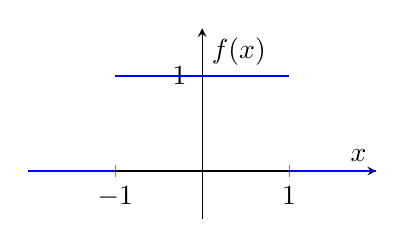
\begin{tikzpicture}
        \begin{axis}[
            axis lines = middle,
            xlabel = $x$,
            ylabel = {$f(x)$},
            ymin=-0.5, ymax=1.5,
            xmin=-2, xmax=2,
            xtick={-1,0,1},
            ytick={0,1},
            samples=100,
            domain=-2:2,
            width=6cm,
            height=4cm
        ]
        \addplot[
            thick,
            blue,
            domain=-1:1,
            samples=100
        ] {1};
        
        \addplot[
            thick,
            blue,
            domain=-2:-1,
            samples=100
        ] {0};
        
        \addplot[
            thick,
            blue,
            domain=1:2,
            samples=100
        ] {0};
        \end{axis}
    \end{tikzpicture}
    \caption{The original function \( f(x) \)}
    \label{fig:3.1}
\end{figure}

\begin{figure}[!h]
    \centering
    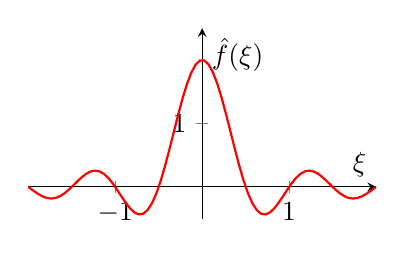
\begin{tikzpicture}
        \begin{axis}[
            axis lines = middle,
            xlabel = $\xi$,
            ylabel = {$\hat{f}(\xi)$},
            ymin=-0.5, ymax=2.5,
            xmin=-2, xmax=2,
            xtick={-1,0,1},
            ytick={0,1},
            samples=200,
            domain=-5:5,
            width=6cm,
            height=4cm
        ]
        \addplot[
            thick,
            red,
            samples=200
        ] {sin(deg(2*pi*x))/(pi*x)};
        \end{axis}
    \end{tikzpicture}
    \caption{The Fourier transform \( \hat{f}(\xi) \)}
    \label{fig:3.2}
\end{figure}

\section{Contour Integration}
A contour integral in the complex plane behaves like a line integral we have studied in calculus. For a path demonstrated as below.
\begin{figure}[!h]
    \centering
    \begin{tikzpicture}
    \begin{axis}[
        axis lines = middle,
        xlabel = {Real},
        ylabel = {Imaginary},
        xmin = 0, xmax = 5,
        ymin = 0, ymax = 5,
        xtick = \empty,
        ytick = \empty,
        width=10cm, height=10cm,
        axis equal
    ]
    
    % Points A and B
    \addplot[
        only marks,
        mark=*,
        mark options={fill=red},
    ] coordinates {(1,2) (4,4)};
    
    % Labels for points A and B
    \node[label={above left:{$A$}},circle,fill,inner sep=1pt] at (axis cs:1,2) {};
    \node[label={above right:{$B$}},circle,fill,inner sep=1pt] at (axis cs:4,4) {};
    
    % Random path from A to B with an arrow
    \addplot[
        thick,
        smooth,
        color=blue,
        -> % Arrow style
    ] coordinates {(1,2) (2,3) (3,2.5) (4,4)};
    
    \end{axis}
    \end{tikzpicture}

    \caption{A path in the complex plane}
    \label{fig:3.3}
\end{figure}
Define a function $f \colon \C \to \C$, and we can integrate the function along this path, written as
\begin{align}
    \int_C f(z) \; dz = \int_{a}^{b} f\paren{z(t)}z'\paren{t}\;dt
\end{align}
It looks like a line integral, and we evaluate it just like a line integral. We would first parameterize the path as a function of time, $z(t)$. And then rewrite the original function as $f\paren{z(t)}$, then multiply it with the derivative of the path. Here are some examples.

\subsubsection{Example 3.3.1}
Let $c$ be the the straight path from $0$ to $1+i$, evaluate
\[
\int_C z^2 \; dz
\]
To solve this, we first parameterize the path. $c \colon z(t) = t + it$ from $t \in \sqbkt{0,1}$. And then we take its derivative.
\[
z'(t) = 1+i
\]
Now, we rewrite the original function $f(z)$ as
\[
f\paren{z(t)} = \paren{t+it}^2
\]
And we can start to evaluate the integral
\begin{align*}
   \int_C z^2 \; dz &= \int_{0}^{1} \paren{t+it}^2\paren{1+i}\;dt\\
                     &= \int_{0}^{1} t^2\paren{1+i}^2\paren{1+i}\;dt \\
                     &= \paren{1+i}^3 \int_{0}^{1} t^2 \; dt\\
                     &= \paren{1+i}^3 \cdot \sqbkt{\left.\frac{1}{3}t^3 \right|_{t=0}^{t=1}}\\
                     &= \frac{\paren{1+i}^3}{2}
\end{align*}

\subsubsection{Example 3.3.2}
Evaluate the integral
\[
\int_C \frac{1}{z}\;dz
\]
Where $c$ is the \textit{positively oriented} unit circle. 

First of all, we find the expression for the path $c \colon z(\theta) = e^{i\theta}$ where $\theta\in\closeopen{0,2\pi}$. Next step we would take the derivative of the path, and it is $z'(\theta) = ie^{i\theta}$

Secondly, we just rewrite the integral as
\begin{align}
   &\int_c \frac{1}{z} \; dz \\
   &= \int_{0}^{2\pi} \frac{1}{e^{i\theta}}\cdot ie^{i\theta} \; d\theta \\
   &= i\int_{0}^{2\pi}  d\theta\\
   &= 2\pi i
\end{align}

\subsubsection{Exercise 3.3.3}
Integrate the following integral over the path $z(\theta) = 6e^{i\theta}+i$
\[
\int_C \frac{1}{z-i} \; dz
\]

\subsubsection{Exercise 3.3.4}
Find 
    \[
    \int_{C} x \; dz
    \]
where $C$ is the directed line segment from the origin to $1+i$.

\subsubsection{Exercise 3.3.5}
Find 
\[
\int_{C} f(z) \; dz
\]
where $f(z) = y-x - 3ix^{2}$ where $C$ is the line from the origin to $i$ followed by the line from $i$ to $1+i$. 

\newpage
\section{Cauchy Integral Formula}
Assume $f(z) = u+iv$ is analytic on $D \subseteq \C$, and assume $C$ is a \textbf{closed curve} around $D$, then 
\begin{align}
    \oint_C f(z) \; dz = 0
\end{align}
The proof of this statement will come later in this note. Here is a graph for visualization. 
\begin{figure}[h!]
    \centering
    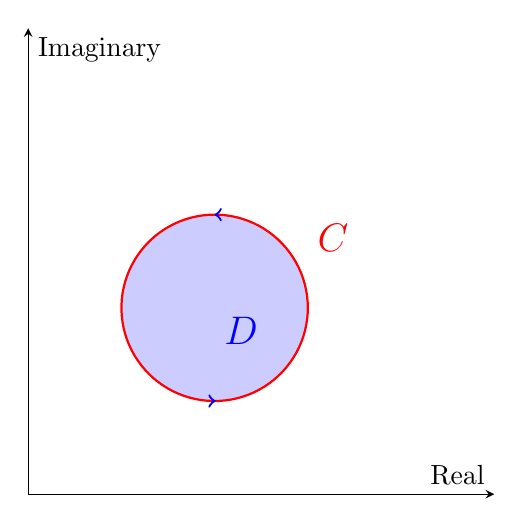
\begin{tikzpicture}
    \begin{axis}[
        axis lines = middle,
        xlabel = {Real},
        ylabel = {Imaginary},
        xmin = 0, xmax = 5,
        ymin = 0, ymax = 5,
        xtick = \empty,
        ytick = \empty,
        width=7.5cm, height=7.5cm,
        axis equal
    ]
    
    % Region D as a filled circle
    \addplot [
        thick,
        domain=0:360,
        samples=100,
        fill=blue!20,
        draw=none,
    ] ({2 + cos(x)}, {2 + sin(x)});
    
    % Closed curve C around D
    \addplot [
        thick,
        color=red,
        domain=0:360,
        samples=100,
    ] ({2 + 1*cos(x)}, {2 + 1*sin(x)});
    
    % Label for region D
    \node at (axis cs:2,2) [below right, color=blue] {\Large $D$};
    
    % Label for closed curve C
    \node at (axis cs:3,3) [below right, color=red] {\Large $C$};

    \addplot[
        thick,
        smooth,
        color=blue,
        -> % Arrow style
    ] coordinates {(2,1) (2.01,1)};

    \addplot[
        thick,
        smooth,
        color=blue,
        -> % Arrow style
    ] coordinates {(2.01,3) (2,3)};

    \end{axis}
    
\end{tikzpicture}
    \caption{A closed curve around $D$}
    \label{fig:3.4}
\end{figure}

For example, the integral
\[
\oint_C \frac{1}{z}\; dz
\]
Will evaluate to $0$ as long as the closed path $C$ does not include the origin where the function is not defined. But if the path $C$ includes the origin, or in other word, the region $D$ bounded by $C$ contains a point where $f(z)= \frac{1}{z}$ is not analytic, then 
\[
\oint_C f(z) \; dz = 2 \pi i
\]
From here, we would introduce the case of the Cauchy integral formula where $D$ contains a point where the function is not analytic. 
\begin{align}
    \oint_c \frac{f(z)}{z-z_0} \; dz = 2\pi i f(z_0)
\end{align} 
Here, $z_0$ is the point where the function is not analytic and inside the region $D$ enclosed by $C$. And this is called the \textbf{Cauchy Integral Formula}.

\subsubsection{Example 3.4.1}
Evaluate the integral, where $c$ is a circle centered at the origin with radius of $5$.
\[
\oint_c \frac{z^2+2z+1}{z(z^2+1)}
\]
To solve this, we need to factor the denominator.
\begin{align*}
     &\oint_c \frac{z^2+2z+1}{z(z^2+1)}\\
    =&\oint_c \frac{z^2+2z+1}{z(z+i)(z-i)}
\end{align*}
We see that the integrand has 3 singularities at $z_1 = 0, z_2 = -1, z_3 = i$. One thing we note is that, if there are multiple singularities, we can define 3 different $f(z)$ and utilize the formula multiple times. For this question, we would define 3 different $f(z)$.
\begin{align*}
    f_1(z) = \frac{z^2+2z+1}{(z+i)(z-i)}\\
    f_2(z) = \frac{z^2+2z+1}{z(z-i)}\\
    f_3(z) = \frac{z^2+2z+1}{z(z+i)}
\end{align*}
Now we make the observation that all 3 singularities are enclosed in the curve $c$, therefore we will take all 3 into account. The integral is evaluated to
\begin{align*}
     &\oint_c \frac{z^2+2z+1}{z(z^2+1)}\\
    =&2\pi i f_1(z_1) + 2\pi i f_2(z_2) + 2\pi i f_3(z_3)\\
    =&2\pi i
\end{align*}
To prove that this methods works require partial faction decomposition and breaking it into different integrals. But it will eventually work out the same way as just adding them together.

\section{Generalized Cauchy Integral Formula}
If we look at the Cauchy integral formula
\[
\oint_c \frac{f(w)dw}{w-z} = 2\pi i f(z)
\]
We can take its derivative on both sides with respect to $z$ as follows
\[
\oint_c \dydx{}{z} \frac{f(w)dw}{w-z} = 2\pi i f'(z)
\]
And this simplifies to
\[
\oint_c \frac{f(w)dw}{(w-z)^2} = 2 \pi i f'(z)
\]
And we can do re-arrange this formula a little to obtain
\begin{align}
    f'(z) = \frac{1}{2\pi i }\oint_c \frac{f(w)}{(w-z)^2}\;dw
\end{align}
We can in fact repeat this process one more time and obtain
\begin{align}
    f''(z) = \frac{1\cdot 2}{2\pi i}\oint_c \frac{f(w)}{(w-z)^3}\;dw
\end{align}
And another
\begin{align}
    f'''(z) = \frac{3!}{2\pi i} \oint_c \frac{f(w)}{(w-z)^4}\;dw
\end{align}
And we can see an obvious trend here, where the $k$-th derivative can be expressed as
\begin{align}
    f^{(k)}(z) = \frac{k!}{2\pi i}\oint_c \frac{f(w)}{(w-z)^{k+1}}\;dw
\end{align}
And this is called the \textbf{Generalized Cauchy Integral Formula}

\section{Laurent Series}

Before delving into \textit{residues}, an important concept we will look at in the next section, it's essential to understand the \textbf{Laurent series}. Given a function \(f(w)\) that is analytic in an annulus \(r_1 < |w - z| < r_2\), the function can be expanded into a Laurent series around \(z\) as:
\[
f(w) = \sum_{n=-\infty}^{\infty} a_n (w - z)^n,
\]
where the coefficients \(a_n\) are given by:
\[
a_n = \frac{1}{2\pi i} \oint_{c} \frac{f(w)}{(w - z)^{n+1}}\, dw,
\]
with \(c\) being a contour within the annulus. You can see this is really similar to the formula we just discussed.

This series generalizes the concept of a \textit{Taylor series} to include terms with negative powers, which are particularly important when dealing with singularities.


The Laurent series expansion of \(f(w)\) is crucial in defining residues. Specifically, the residue of \(f(w)\) at \(z\) is the coefficient \(a_{-1}\) in the Laurent series:
\[
\text{Res}(f, z) = a_{-1} = \frac{1}{2\pi i} \oint_{c} \frac{f(w)}{w - z} \, dw.
\]
Where $\text{Res}(f,z)$ means the residue of the function $f$ at $z$. 

\section{Residue}

Now that we have established the Generalized Cauchy Integral Formula and the Laurent series, we can utilize this knowledge to introduce the concept of \textbf{residues} in complex analysis.

The residue of a function \(f(w)\) at a point \(z\) is closely related to the value of a contour integral involving \(f(w)\). Specifically, the residue is the coefficient of \(\frac{1}{w - z}\) in the Laurent series expansion of \(f(w)\) around \(z\).


Using the Generalized Cauchy Integral Formula, we observe that when \(k = 0\), the formula reduces to the classic Cauchy Integral Formula:
\[
f(z) = \frac{1}{2\pi i} \oint_c \frac{f(w)}{w - z} \, dw.
\]
Here, the integral represents the residue of \(\frac{f(w)}{w - z}\) at \(w = z\).

For \(k = 1\), we obtained:
\[
f'(z) = \frac{1}{2\pi i} \oint_c \frac{f(w)}{(w - z)^2} \, dw.
\]
This integral can be interpreted as involving the residue of \(\frac{f(w)}{(w - z)^2}\).

Thus, the residues provide a way to calculate the integral of meromorphic functions around isolated singularities. In particular, for a meromorphic function \(g(w) = \frac{f(w)}{(w - z)^{k+1}}\), the residue at \(z\) contributes directly to the value of the integral. This observation leads us naturally to define the residue:
\[
\text{Res}(f, z) = \frac{1}{2\pi i} \oint_c \frac{f(w)}{w - z} \, dw,
\]
where \(c\) is a small contour around \(z\).

Residues play a central role in evaluating contour integrals, particularly in cases where the integrand has poles. They allow us to compute integrals over complex contours more efficiently and are the foundation of many powerful theorems, such as the \textbf{Residue Theorem}.

\subsubsection{Meromorphic Functions}
A Meromorphic is a complex function that is holomorphic everywhere except for some isolated singularity in $D$. Think of it as a function that is very nice except for at a particular point such as $f(x) = \frac{1}{x^2}$ at $x=0$ in our good-old real function. 

\section{Residue Theorem}

The Residue Theorem states that if \(f(w)\) is a meromorphic function with isolated singularities inside a contour \(c\), the integral of \(f(w)\) around \(c\) is \(2\pi i\) times the sum of the residues of \(f(w)\) at those singularities:
\[
\oint_c f(w) \, dw = 2\pi i \sum \text{Res}(f, z_i),
\]
where \(z_i\) are the isolated singularities of \(f(w)\) inside \(c\).

With the understanding of this Theorem, you can now see why the method we used to integrate in \textit{Example 3.4.1} worked as it is. 







\end{document}

